\chapter{Saliency Maps}
\label{cha:saliency}

\section{Konzept}
Ein verbreitetes Verfahren aus dem Bereich Computer Vision zur Visualisierung relevanter Pixel ist die Erstellung von Saliency Maps (dt. Ausprägungskarten). Diese können verwendet werden, um die Qualität, sprich Aussagekraft, jedes einzelnen Bildpunkts ersichtlich zu machen. Simonyan et al. \cite{simonyan_deep_2013} führt die grundlegende Methodik entsprechend Saliency Maps weiter aus und unterscheidet zwischen einer allgemeinen “Klassen-Definierenden” Saliency Map sowie einer Saliency Map zu einem gegebenen Eingabebild entsprechend der Zielklassen.


Gebräuchliche Anwendung dieses Verfahrens im Machine Learning Bereiches betreffen der Darstellung von High level Features einzelner Neuronen \cite{liu_delving_2016} im bezug auf eine gezielte Klasse. Diesen Ansatz weiterverfolgend, entsprechen die erzeugten Saliency Maps im letzten Layer einer starken Neuronenaktivierung, die einer “high level” darstellung der gezielten klasse entspricht, die vom NN für das Bild errechnet wurde. 


Diese Saliency Map sollte also im Rückschluss mit einer hohen Koinzidenz bezüglich der entsprechende Klasse klassifiziert werden, wenn das erzeugte Bild als Eingabe verwendet wird. Daraus ergibt sich die Hypothese, mithilfe dieser Visualisierung für den menschen semantisch nicht erkennbare Verkehrszeichen Bilder zu erzeugen, die hohe Zielkonfidenzen mit $90\%$ oder mehr erreichen. Die beschriebene Methode wird in der Implementierung als “Vanilla Saliency” bezeichnet.

\section{Implementierung}

Die Verfahren zur Erzeugung der Saliency Maps setzen eine identische Datenvorverarbeitung voraus. 
Die Trainingsbilder des GTSRB Datensatz wurden konvertiert und entsprechend der Eingabeparameter des Aphrodite-Modells als PNG mit Größe $64 \times 64 $ im Dateisystem abgespeichert.

Nachfolgend wird der vollständige Datensatz lokal am eigenen Modell klassifiziert und alle Bilder mit einer Konfidenz von 100\% separat gesammelt. 

Die vorgestellten Verfahren Vanilla Saliency\cite{simonyan_deep_2013}, Guided Backpropagation[] und Integrated Gradient[] werden jeweils in einer ungefilterten und und geglätteten Variante verwendet entsprechend einer auf die Aufgabenstellung angepasster Implementation auf der Basis von [https://github.com/experiencor/deep-viz-keras]. 

Ausgegeben wird ein Graustufenbild in der die relevanten Pixelbereiche durch hellere Einfärbung gekennzeichnet werden.

Diese Bilder wurden danach an das Trasi webinterface geschickt und das Resultat der prediction abgespeichert. Zusätzlich wird pro Verfahren ein Logfile erstellt, welches alle Bilder mit einer Konfidenz >0.9 sowie die geschätzte Klasse und das Ursprungsbild festhält.
%
%vanilla 58 p min
%smooth vanilla 37 p m
%
%integrated gradient 56 p m
%smooth intr grad 34 p m
%
%
%guided Backprop: 46 p min bild
%smoothed Guided Backprop 25 p min  


\section{Ergebnisse}

Aus der Implementation konnten folgende Ergebnisse zu den 6 vorgestellten Variationen gesammelt werden. 

Alle ungeglätteten Verfahren konnten keine positiven Ergebnisse bezüglich der Bilderzeugung mit einer Konfidenz $> 0.9$ liefern. Dies lässt sich möglicherweise auf die besonderen Einschaften von CNNs zurückführen, dass ohne Glättung in dem - ohne farbchannel - bereits dimensionsreduziertem Bild keine ausgeprägten Kanten vorhanden sind und nach dem "Falten" Informationen verloren gehen. Desweiteren konnte am Blackbox Modell beobachtet werden, dass alle erzeugten ungegeglätteten Saliency Maps mit einer Konfidenz von $0.45834911$ als Klasse "Baustelle" erkannt werden.

Dahingegen konnten bei allen geglätteten Varianten Bilder erzeugt werden, die vom Blackboxmodell mit hoher Sicherheit eine Klasse zugeordnet wurden. Es konnten einige unerwarteten Anomalien bei der Klassifizierung am Fremdmodell beobachtet werden.  Tabelle \ref{tab:sal1} zeigt wie aus Bild \ref{fig:salUrsprung} (Höchstgeschwindigkeit (30))  mit den Verfahren "Smoothed Guided Backpropagation" (vgl. []) und "Smoothed Vanilla Saliency" (vgl. []) ein Bild erzeugt, welche mit einer Konfidenz >0.9 vom Webinterface erkannt wurden. Dabei muss beachtet werden, dass die Bilder als unterschiedliche Klassen eingestuft wurden. "Vanilla Saliency" stimmt überein (Höchstgeschwindigkeit (30), Konfidenz 0.9283), "Guided Backpropagation" wurde vom Fremdmodell einer anderen Klasse zugeordnet (Überholverbot, Konfidenz 0.9155).

\begin{table}
	\centering
	\begin{tabular}{p{4.4cm}p{4.4cm}p{4.4cm}}
		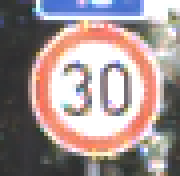
\includegraphics[width=\linewidth]{Images/AnPe/10771} \label{fig:salUrsprung}& 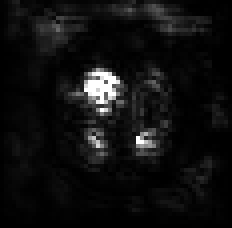
\includegraphics[width=\linewidth]{Images/AnPe/10771_guided} &
		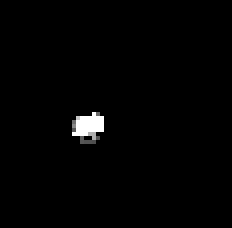
\includegraphics[width=\linewidth]{Images/AnPe/10771_vanil}\\ 
		Ursprungsbild & Guided Backprop. & Vanilla Saliency \\
		Höchstgeschwindigkeit (30) & Überholverbot & Höchstgeschwindigkeit (30)\\
		& 0.9155 & 0.9283\\
		
	\end{tabular} 

	\caption{Ergebnisse von verschiedenen Verfahren am selben Bild. }
	\label{tab:sal1}
\end{table}

%\begin{figure}
%	\begin{subfigure}{.33\textwidth}
%		\centering
%		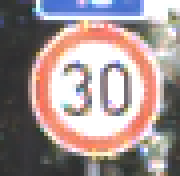
\includegraphics[width=.8\linewidth]{Images/AnPe/10771}
%		\caption{Ursprungsbild (Höchstgeschwindigkeit 30)}
%		\label{fig:ursprung1}
%	\end{subfigure}%penis
%	\begin{subfigure}{.33\textwidth}
%		\centering
%		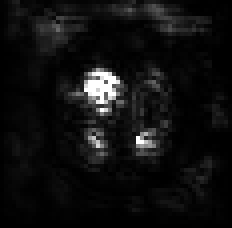
\includegraphics[width=.8\linewidth]{Images/AnPe/10771_guided}
%		\caption{Halblabor.}
%		\label{fig:salmap1}
%	\end{subfigure}
%	\begin{subfigure}{.33\textwidth}
%		\centering
%		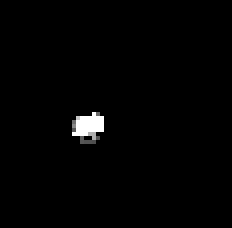
\includegraphics[width=.8\linewidth]{Images/AnPe/10771_vanil}
%		\caption{Freie Umgebung.}
%		\label{fig:salmap_1}
%	\end{subfigure}
%\end{figure}

Tabelle \ref{tab:sal2} zeigt weitere Beispiele für erfolgreiche Saliency Maps. Wieder kann beobachtet werden, dass Bilder nicht mehr der ursprünglichen Klasse zugeordnet werden, aber trotzdem Konfidenzen >0.9 erreicht wurden. 


\begin{table}
	\centering
	\begin{tabular}{p{4.4cm}p{4.4cm}}
		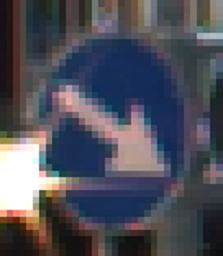
\includegraphics[height=4.4cm]{Images/AnPe/11240} &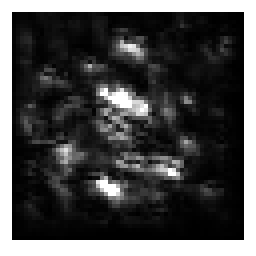
\includegraphics[width=\linewidth]{Images/AnPe/11240_guided}  \\
		Rechts Vorbei & Einmalige Vorfahrt\\
		& 0.9678\\
		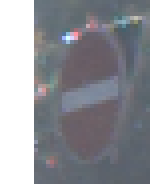
\includegraphics[height=4.4cm]{Images/AnPe/06848} &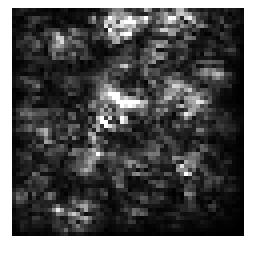
\includegraphics[width=\linewidth]{Images/AnPe/06848_s_int}  \\
		Einfahrt Verboten & Überholverbot\\
		& 0.9571\\
		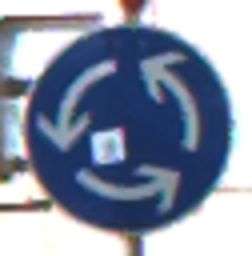
\includegraphics[height=4.4cm]{Images/AnPe/04709} &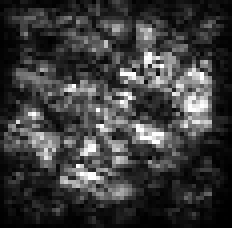
\includegraphics[width=\linewidth]{Images/AnPe/04709_int_grad}  \\
		Kreisverkehr &Baustelle \\
		& 0.9999
	\end{tabular}
	\caption{Ergebnisse von verschiedenen Verfahren am selben Bild. }
\label{tab:sal2}
\end{table}

Zusammenfassend konnte gezeigt werden, dass es mithilfe der Erstellung von Saliency Maps an einem eigenen Modell Bilder erzeugt werden können, welche von einem unbekanntem NN mit hohen Konfidenzen verschiedenen Klassen zugeordnet werden. Die Erfolgsrate in Relation zur Anzahl erzeugter Bilder und dem Rechenaufwand ist dabei jedoch gering und es herrscht aktuell keine Aussagekraft darüber, welcher Klasse das erzeugte Bild zugeordnet wird. 
